The world in which we live is known more to us than is the universe or, perhaps, universes in which it exists.  This world is known to be part of a solar system which is known to be part of a universe made up of similar solar systems and galaxies.  We know more about the world in which we live than we do about the universe in which it resides.  In fact, the purposes of this textbook are realized independent of knowing any more of a universal nature extant above and beyond our world.

The primary purpose of this textbook may be addressed directly by recognizing the ultimate system of interest in STEA to be \textit{the world in which we live}.  We observe the \textit{natural}, the \textit{human-made}, and the \textit{human-modified} worlds to be interconnected sectors as illustrated in \Cref{fig:humanModifiedVennDiagram}.  Of these, it is the human-modified world that should be adopted as the highest-level system of our concern, because that is where we actually live.

\begin{figure}[h]
\centering
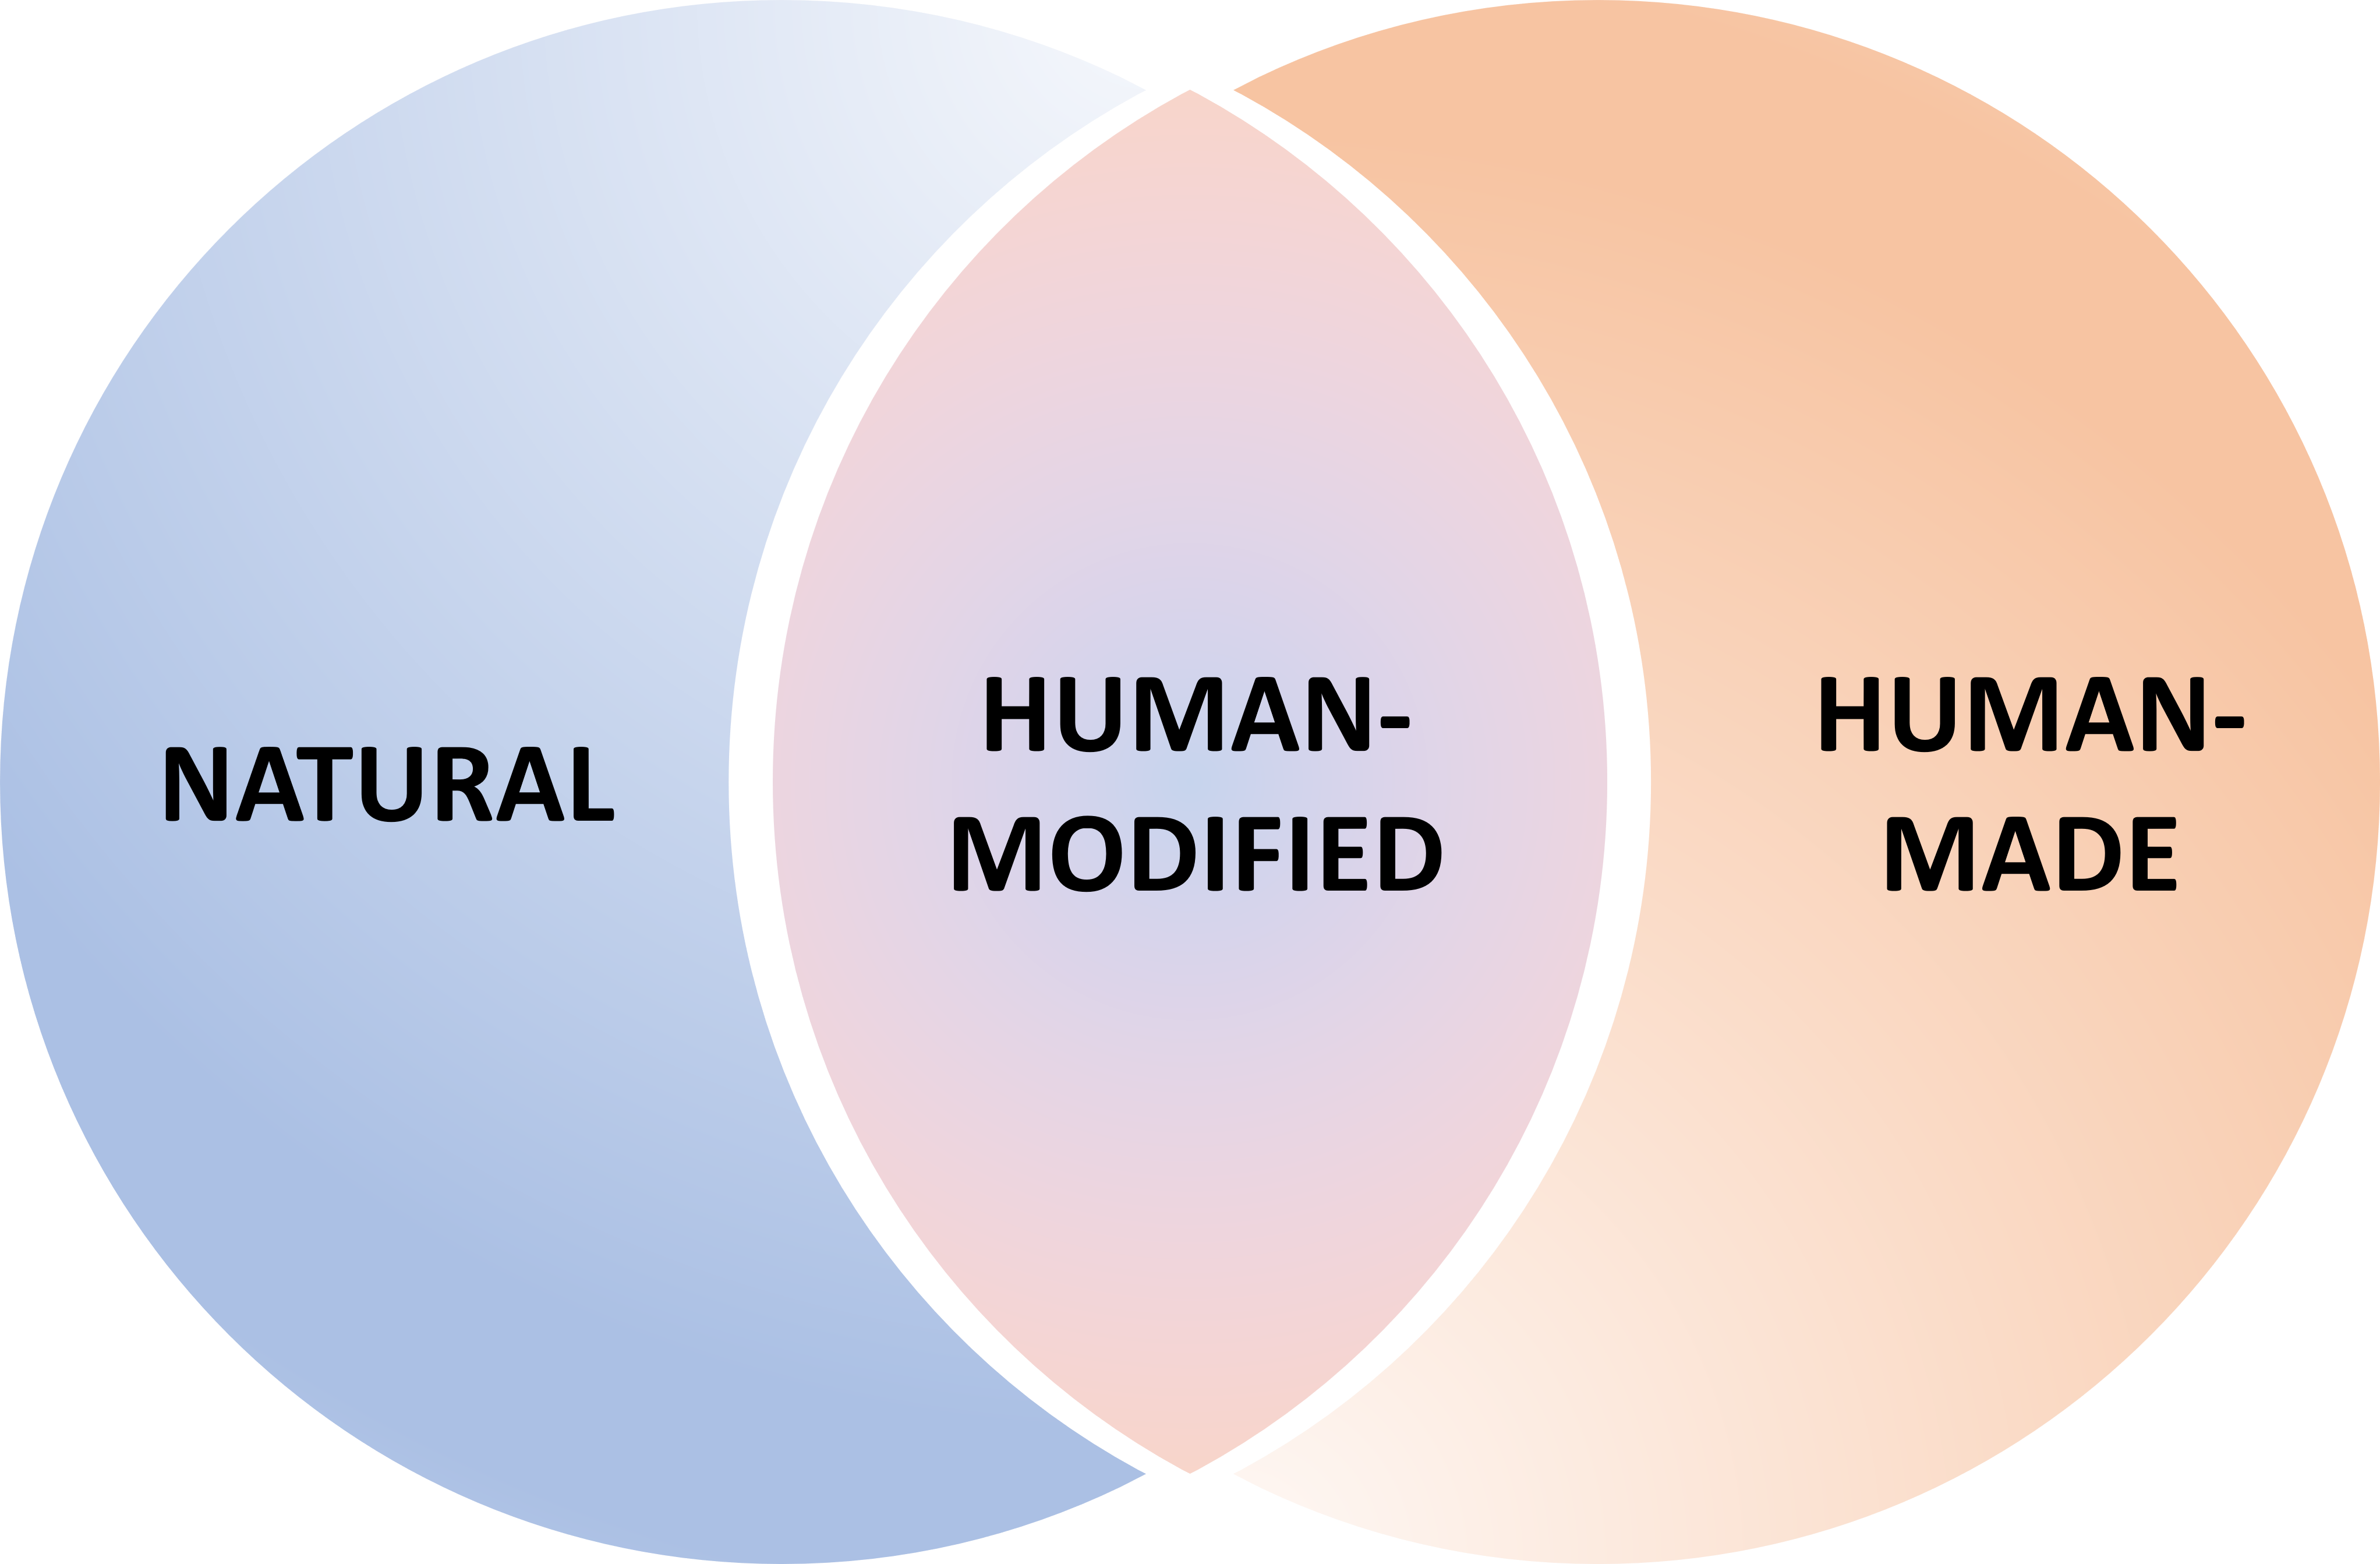
\includegraphics[width=0.9\textwidth]{humanModifiedVennDiagram.png}
\caption{Our world viewed as interconnected sectors.}
\label{fig:humanModifiedVennDiagram}
\end{figure}

The natural world came into being by natural processes.  The human-made world is made up of systems and products that resulted from the intervention of humans through components, attributes, and relationships.  The \textit{human-modified world} is the natural world into which the human-made has been introduced as systems, subsystems, entities, and artifacts; a world becoming increasingly complex.  This book strives to justify the human-modified world as the ultimate system level at which the viability of all that is human made should be judged.